
\begin{figure}[h!]
\begin{LineCode}[commandchars=\*\[\]]
type edge(node, node).*hfill// Predicate declaration
type linear visit(node).
type linear unvisited(node).
type linear visited(node).

visit(A), *label[line:language:visit_first1]*hfill // Rule 1: visit node
unvisited(A) -o
   visited(A),
   {B | !edge(A, B) -o visit(B)}.*label[line:language:visit_first2]*label[line:language:visit_comprehension]

visit(A),*label[line:language:visit_second1]*hfill // Rule 2: node already visited
visited(A)
   -o visited(A).*label[line:language:visit_second2]
\end{LineCode}
  \mycap{LM code for the graph visit program.}
  \label{code:language:visit}
\end{figure}

Our third example, shown in Fig.~\ref{code:language:visit}, presents another LM
program that, for a given graph of nodes, performs a visit to all nodes
reachable from node \code{@1}. The first rule of the program
(lines~\ref{line:language:visit_first1}-\ref{line:language:visit_first2}) visits
node \code{A} for the first time: fact \code{visited(A)} is derived and a
\emph{comprehension} construct is used to go through all the edge facts and then
derive \code{visit(B)} at each neighbor node \code{B}. The second rule of the
program
(lines~\ref{line:language:visit_second1}-\ref{line:language:visit_second2})
applies when the node is already visited more than once: we keep the
\code{visited} fact and delete \code{visit}. The initial facts shown in
Fig.~\ref{code:language:visit_initial} use the \code{visit(@1)} fact to start
the program.

\begin{figure}[h!]
\begin{LineCode}[commandchars=\*\[\]]
!edge(@1, @2).
!edge(@1, @4).
!edge(@2, @3).
!edge(@2, @4).
!edge(@2, @1).
!edge(@3, @2).
!edge(@4, @1).
!edge(@4, @2).

unvisited(@1).
unvisited(@2).
unvisited(@3).
unvisited(@4).

visit(@1).
\end{LineCode}
  \mycap{Initial facts for the graph visit program. Nodes reachable from node \code{@1} will be marked as \code{visited}.}
  \label{code:language:visit_initial}
\end{figure}

\begin{figure}[h]
        \centering
        \begin{subfigure}[b]{0.45\textwidth}
                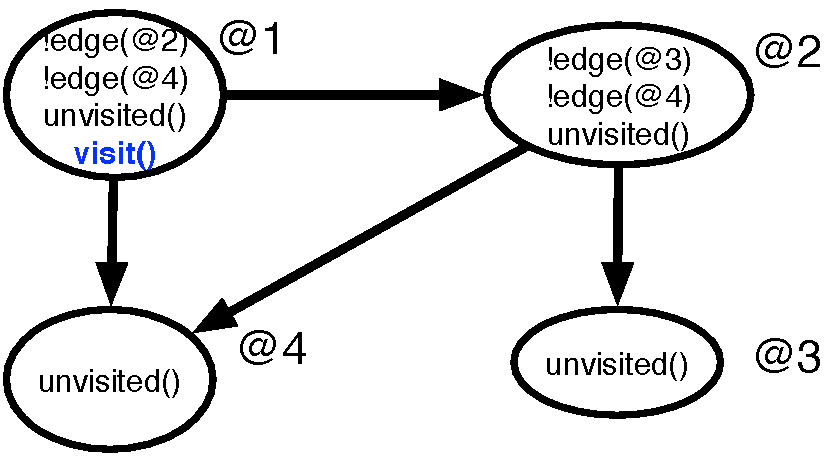
\includegraphics[width=\textwidth]{figures/visit/trace1}
                \mycap{Initial database.}
                \label{fig:exec_trace1}
        \end{subfigure}%
        ~ %add desired spacing between images, e. g. ~, \quad, \qquad etc.
          %(or a blank line to force the subfigure onto a new line)
        \begin{subfigure}[b]{0.45\textwidth}
                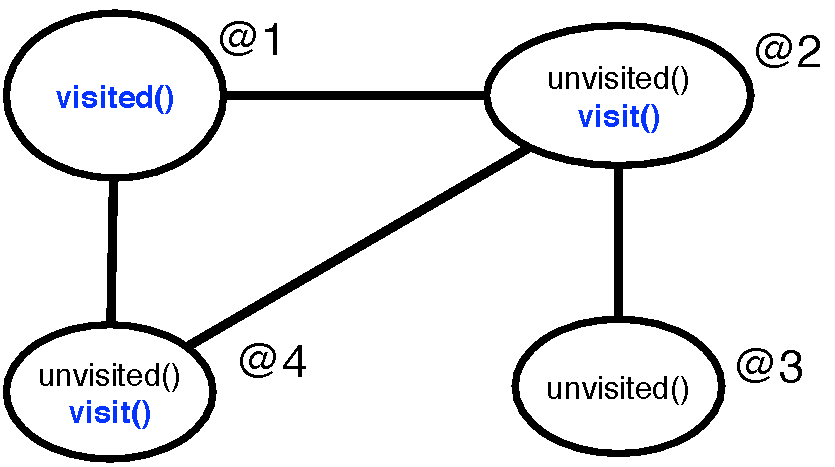
\includegraphics[width=\textwidth]{figures/visit/trace2}
                \mycap{After applying rule 1 at node \code{@1}.}
                \label{fig:exec_trace2}
        \end{subfigure}\\
        \begin{subfigure}[b]{0.45\textwidth}
                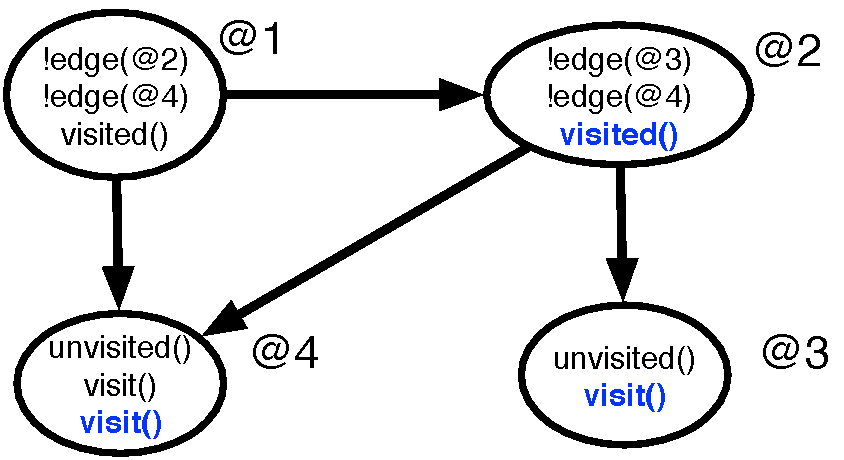
\includegraphics[width=\textwidth]{figures/visit/trace3}
                \mycap{After applying rule 1 at node \code{@2}.}
                \label{fig:exec_trace3}
        \end{subfigure}%
        ~ %add desired spacing between images, e. g. ~, \quad, \qquad etc.
         %(or a blank line to force the subfigure onto a new line)
        \begin{subfigure}[b]{0.45\textwidth}
                  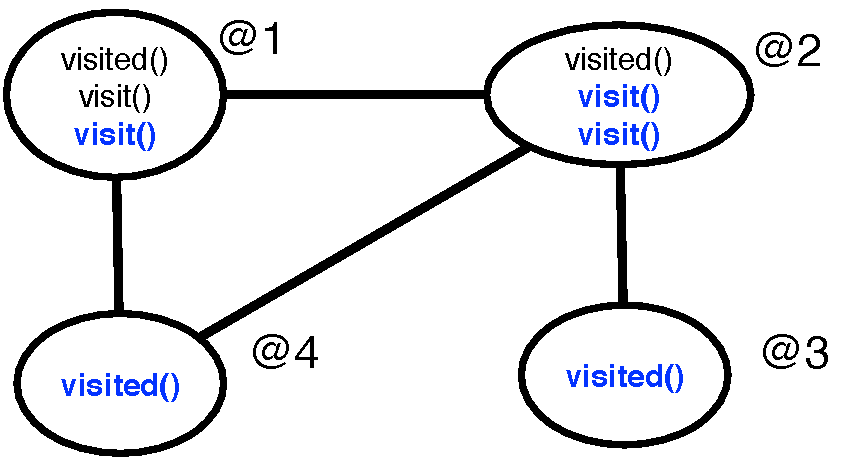
\includegraphics[width=\textwidth]{figures/visit/trace4}

                  \mycap{After applying rule 1 and 2 at node \code{@4} and
                  rule 1 at node \code{@3}.}

                  \label{fig:exec_trace4}
          \end{subfigure}
        \mycap{A possible execution trace for the visit
           program. Note that the \code{edge} facts were omitted for simplicity.}
        \label{fig:exec_trace}
\end{figure}

Fig.~\ref{fig:exec_trace} shows a possible execution trace for the visit
program. After applying the first rule at node \code{@1} we get the database in
Fig~\ref{fig:exec_trace}~(b).  Note that node \code{@1} is now visited and nodes
\code{@2} and \code{@4} now have a \code{visit} fact. At this point, we could
either apply rule 1 at node \code{@2} or at node \code{@4}.  For this specific
trace, we apply the rule at node \code{@2}, resulting in
Fig.~\ref{fig:exec_trace}~(c). Node \code{@4} now has two \code{visit} facts,
thus we can apply rule 1 followed by rule 2, therefore consuming both
\code{visit} facts and deriving \code{visited}. In addition, we can also apply
rule 1 at node \code{@3} to reach the state of Fig.~\ref{fig:exec_trace}~(d).

The graph visit has the potential to have plenty of concurrency. Once the visit
starts from the initial node, it expands to other nodes, allowing several nodes
to derive rules concurrently. At some point, the amount of concurrency is
reduced because more and more nodes have been visited. The level of concurrency
depends on the structure of the graph. In the worst case, if the graph is a
chain of nodes then the program becomes effectively sequential.  In the best
case, if the graph is densely connected (each node connects to most nodes in the
graph), then it is possible to run the program on most nodes at the same time.

The goal of introducing higher-level declarative languages is to facilitate
reasoning about the properties of a program. In the case of the visit program,
the most important goal is to prove that, if the graph is connected, then all
the nodes will become \code{visited}, regardless of the order in which we apply
the rules. First, we define a visit graph:

\begin{definition}[Visit graph]
A visit graph is an ordered pair $G = (N, E)$ comprising a set $N$ of nodes together
with a set $E$ of edges. Set $E$ contains pairs $(A, B)$ that correspond to
facts $\bang \mathtt{edge}(A, B)$. For every pair $(A, B) \in E$ there is also a
pair $(B, A) \in E$, representing an undirected edge.
\end{definition}

To prove the correctness property of the program, we first define the main
\emph{invariant} of the program:

\begin{invariant}[Node state]
A node is either \code{visited} or \code{unvisited} but not both.
\end{invariant}

\begin{proof}

From the initial facts we check if all nodes start as \code{unvisited}. This is
clearly true for the previous example. Rule 1 changes a node from
\code{unvisited} to \code{visited}, while rule 2 keeps the node \code{visited},
proving the invariant.

\end{proof}

Invariants are conditions that never change, no matter which rules are derived
during execution. With this invariant, it is now possible to classify nodes of
the graph $G$ according to their state:

\begin{definition}[Node sets] \code{visited} nodes are contained in set $V$,
while \code{unvisited} nodes are in set $U$. From the node state invariant, we
know that $V \cup U = N$ and $V \cap U = \emptyset$.
\end{definition}

We can now prove an important lemma about sets $V$ and $U$:

\begin{invariant}[Visited set]

After each rule derivation, visited set $V$ always increases or stays the same
size. The inverse is true for set $U$.

\end{invariant}
\begin{proof}
Initially, $V = \emptyset$ and $U = N$.
By rule 1, $V$ increases by 1 while $U$ decreases by 1. With rule 2, set
membership remains unchanged.
\end{proof}

In turn, since set membership changes from $U$ to $V$, we now prove the
following:

\noindent\begin{minipage}{\linewidth}
\begin{lemma}[Edge visits]\label{lemma:language:edge_visits}
The program generates at most one \code{visit} per directed edge and for a node
$a \in N$ that receives a \code{visit} fact, then for all $b \in N$ where $(a,
b) \in E$, exactly one \code{visit} fact is generated at $b$.
\end{lemma}
\end{minipage}
\begin{proof}
From the visited set invariant, we know that once nodes become members of set $V$,
they no longer return to set $U$, therefore rule 1 applies once per
node. This rule generates a \code{visit} fact per neighbor node.
\end{proof}

In order to prove that all the nodes in the graph are visited, we need to make
sure that the graph is connected.

\begin{definition}[Connected graph]
A connected graph is a graph where every pair of nodes has a path between them.
\end{definition}

Finally, we prove that all nodes will become \code{visited}.

\begin{theorem}[Graph visit correctness]
If graph $G$ is connected, set $V$ will eventually include all nodes in $N$,
while $U = \emptyset$.
\end{theorem}
\begin{proof}
Proof by induction.

\begin{itemize}

   \item Base case: initial fact \code{visit(@1)} adds node \code{@1} to $V$.
      By Lemma~\ref{lemma:language:edge_visits}, a \code{visit} fact is generate
      for all edges of \code{@1}.

   \item Inductive case: assume visited set $V'$ and unvisited set $U'$.
  Since the graph
   is connected, there must be a node $a \in V'$ that is connected to a node $b
   \in U'$. Using the Edge visits lemma, a $\mathtt{visit}(b)$ fact is generated,
   swapping $b$ from $U'$ to $V'$.
\end{itemize}

Eventually, set $V$ will include all nodes in $N$. Otherwise, there would be
unreachable nodes in the graph and that would be a contradiction since the graph
is connected.
\end{proof}

